\documentclass[english,10pt]{beamer}


\usepackage{amsmath,amssymb,amsthm,bbm}
\usepackage{graphicx,transparent,eso-pic}
\usepackage[document]{ragged2e}
\usepackage{pagecolor,color,ulem,soul}



\usetheme{Boadilla}

%\setbeamertemplate{footline}[text line]{}
%\setbeamercolor{structure}{fg=purple!50!blue, bg=purple!50!blue}

% cybergeo palette (from Clem server)
% #1C6F91, "#df691a", "#77c5ba", "orange", "#2db92d", "#e1ff2f", "#ff2313", "#bbab61
% redefine palette
\definecolor{cybblue}{HTML}{1C6F91}
\definecolor{cyborange}{HTML}{DF691A}
\definecolor{cybbluegreen}{HTML}{77C5BA}
\definecolor{cybgreen}{HTML}{2DB92D}
\definecolor{cybgreenyellow}{HTML}{E1FF2F}
\definecolor{cybred}{HTML}{FF2313}
\definecolor{cybglaucous}{HTML}{BBAB61}


\setbeamercolor{structure}{fg=cybblue}
\setbeamercolor{footline}{fg=orange, bg=orange}

\setbeamercovered{transparent}


%\addtobeamertemplate{title page}{%\hspace{-0.4cm}
%
%}{%
%\begin{textblock*}{150mm}(-1cm,-1.5cm)
%\end{textblock*}
%}



%\vspace{-0.1cm}
\addtobeamertemplate{frametitle}{\hspace{-0.4cm}
\includegraphics[width=1.08\textwidth]{figures/cybergeo30_template_bandeau-haut}
}{%
%\begin{textblock*}{150mm}(-1cm,-1.5cm)
%\end{textblock*}
}


% shortened command for a justified frame
\newcommand{\jframe}[2]{\frame{\frametitle{#1}\justify{#2}}}


\newcommand{\noun}[1]{\textsc{#1}}
\newcommand{\jitem}[1]{\item \begin{justify} #1 \end{justify} \vfill{}}
\newcommand{\sframe}[2]{\frame{\frametitle{#1} #2}}

\DeclareMathOperator{\Cov}{Cov}
\DeclareMathOperator{\Var}{Var}
\DeclareMathOperator{\E}{\mathbb{E}}
\DeclareMathOperator{\Proba}{\mathbb{P}}

\newcommand{\Covb}[2]{\ensuremath{\Cov\!\left[#1,#2\right]}}
\newcommand{\Eb}[1]{\ensuremath{\E\!\left[#1\right]}}
\newcommand{\Pb}[1]{\ensuremath{\Proba\!\left[#1\right]}}
\newcommand{\Varb}[1]{\ensuremath{\Var\!\left[#1\right]}}

% norm
\newcommand{\norm}[1]{\| #1 \|}

\newcommand{\indep}{\rotatebox[origin=c]{90}{$\models$}}


\usepackage{textpos}



\begin{document}


% Le journal Cybergeo a implémenté depuis une dizaine d'années des initiatives complémentaires pour une science ouverte appliquée : les rubriques DataPapers et GeOpenMod pour l'ouverture et le partage des données et modèles, et la plateforme CybergeoNetworks pour une exploration réflexive du corpus de la revue par les auteurs, éditeurs, et lecteurs. Cette présentation reviendra sur leur mise en place et leur suivi, puis discutera la perspective d'une intégration plus forte entre ces différentes composantes d'une science ouverte au sein du journal.



\title{\phantom{}\vspace{2cm}\phantom{}\\Reproductibilité et réflexivité : l'ambition de Cybergeo pour une Science Ouverte appliquée}


\author{\vspace{-1.5cm}\\Juste Raimbault$^{1,2,3,4}$}


\institute{\vspace{-0.5cm}\\$^{1}$LaSTIG, Universit{\'e} Gustave Eiffel, IGN-G{\'e}odata Paris\\
$^{2}$CASA, University College London\\
$^{3}$UAR 3611 ISC-PIF\\
$^{4}$UMR CNRS 8504 G{\'e}ographie-cit{\'e}s}

\date{Les 30 ans de Cybergeo : 1996-2026}


\usebackgroundtemplate{

\includegraphics[width=1.06\textwidth]{figures/cybergeo30_template_title_haut}}


{
\setbeamertemplate{footline}{\vspace{-2cm}
\includegraphics[width=1.06\textwidth]{figures/cybergeo30_template_title_bas}}
\begin{frame}
\titlepage
\end{frame}
}

\usebackgroundtemplate{}

\setbeamertemplate{footline}{\vspace{-2cm}\hspace{-0.4cm}
\includegraphics[width=1.04\textwidth]{figures/cybergeo30_template_bandeau-bas}}


\section{Introduction}


\begin{frame}
\frametitle{Cybergeo pionnier de la science ouverte}

\vspace{-0.8cm}

\begin{itemize}
	\item Création en 1996 par Denise Pumain, première revue en ligne en SHS
	\item Accès entièrement ouvert, pas de coût pour les auteurs
\end{itemize}

\begin{center}
	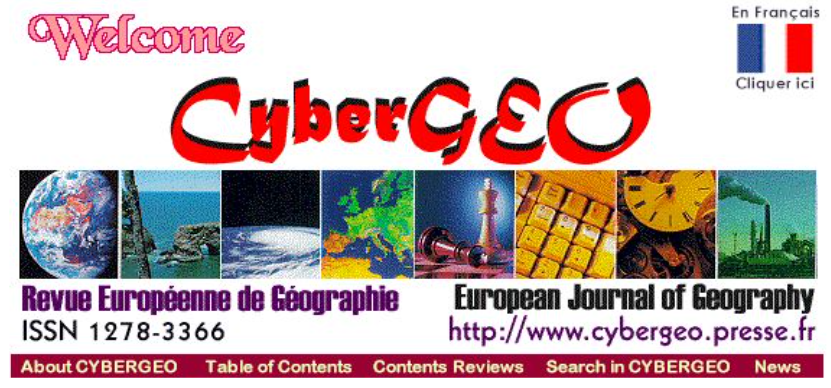
\includegraphics[width=0.6\linewidth]{figures/cyb_vintage}
\end{center}

\footnotesize

\textit{Source : capture webarchve du 12 décembre 1998\\\url{https://web.archive.org/web/19981212024153/http://www.cybergeo.presse.fr/}}

\end{frame}



\begin{frame}
\frametitle{Histoire de Cybergeo}

% 2007 OpenEditions
% 2011 Freemium

\begin{itemize}
	\item 2007 : rejoint \texttt{revues.org}, en même temps que la création du Centre pour l’édition électronique ouverte (mentionné comme ``Grande date'' dans l'histoire d'OpenEditions)
	\bigskip
	\item 2008 : lancement du projet JournalBase par Christine Kosmopoulos (recensement des revues en SHS et de leur référencement)
	\bigskip
	\item 2011 : passage en abonnement Freemium, modèle diamant snas coût pour le lecteur ni l'auteur et en licence CC-BY
	\bigskip
	\item 2018 : blog Cybergeo Conversation
\end{itemize}

\end{frame}




\section{Data et Model papers}



\begin{frame}
\frametitle{Rubrique GeOpenMod}

\textbf{Rubrique fondée en 2014 par Arnaud Banos pour encourager l'ouverture des modèles et logiciels en géographie} \cite{banos2014presentation}

\bigskip
\bigskip

% citations : 0+0+4+5+1+9+11+5+13+7+4+4+12+8+12=

\begin{itemize}
	\item 16 articles publiés (4 en cours d'évaluation), 95 citations
	\item évaluation du code et tests de reproductibilité
	\item ouverture du code (licence ouverte, git)
	\item principes FAIR for Research Software
	\item description standardisée du modèle (ODD, UML)
\end{itemize}


\end{frame}



\begin{frame}
\frametitle{Rubrique Data Papers}

% citations : 24+22+22+6+55+14+7+3+20+2+2+1+4+0+0=

\textbf{Rubrique fondée en 2017 pour encourager l'ouverture des données}

\cite{cybergeo2017presentation}

\bigskip
\bigskip


\begin{itemize}
	\item 16 articles publiés (3 en cours d'évaluation), 182 citations
	\item spécifique aux données géospatiales
	\item partage des données sur un dépôt extérieur, principes FAIR
	\item métadonnées spécifiques : type de représentation, échelle ou résolution, étendue géographique, CRS
\end{itemize}

\end{frame}


\begin{frame}
\frametitle{Expérience d'édition GeOpenMod et Data papers}

\textbf{Rubriques dynamiques au contenu varié, répondent aux attentes des communautés et des auteurs}

\medskip

\textbf{Difficultés :}

\begin{itemize}
	\item redondance avec des articles standard
	\item anonymisation de la soumission
\end{itemize}


\textbf{Perspectives :}

\begin{itemize}
	\item évolution des consignes de soumission, des dépôts recommandés, possible suppression de l'anonymat
	\item pour les modèles, étape supplémentaire de validation et d'analyse de sensibilité : instances OpenMOLE \cite{reuillon2013openmole} dédiées mises à disposition des auteurs
\end{itemize}

\end{frame}



\section{Reflexivité : CybergeoNetworks}




\begin{frame}
\frametitle{Explorateur de corpus CybergeoNetworks}


% cybergeo20
% prototype pour les 20 ans
% mentionner // David OpenJournalScope ; développements en cours

Pour l'anniversaire des 20 ans de Cybergeo en 2016, réalisation d'une \textbf{application web} d'exploration du \textbf{corpus de la revue et de son voisinage scientifique} : \url{https://analytics.huma-num.fr/geographie-cites/cybergeonetworks/}

\smallskip

$\rightarrow$ \textbf{Extensions en cours :} mise à jour du corpus pour les 30 ans ; projet OpenJournalScope en lien avec Gargantext

\begin{center}
	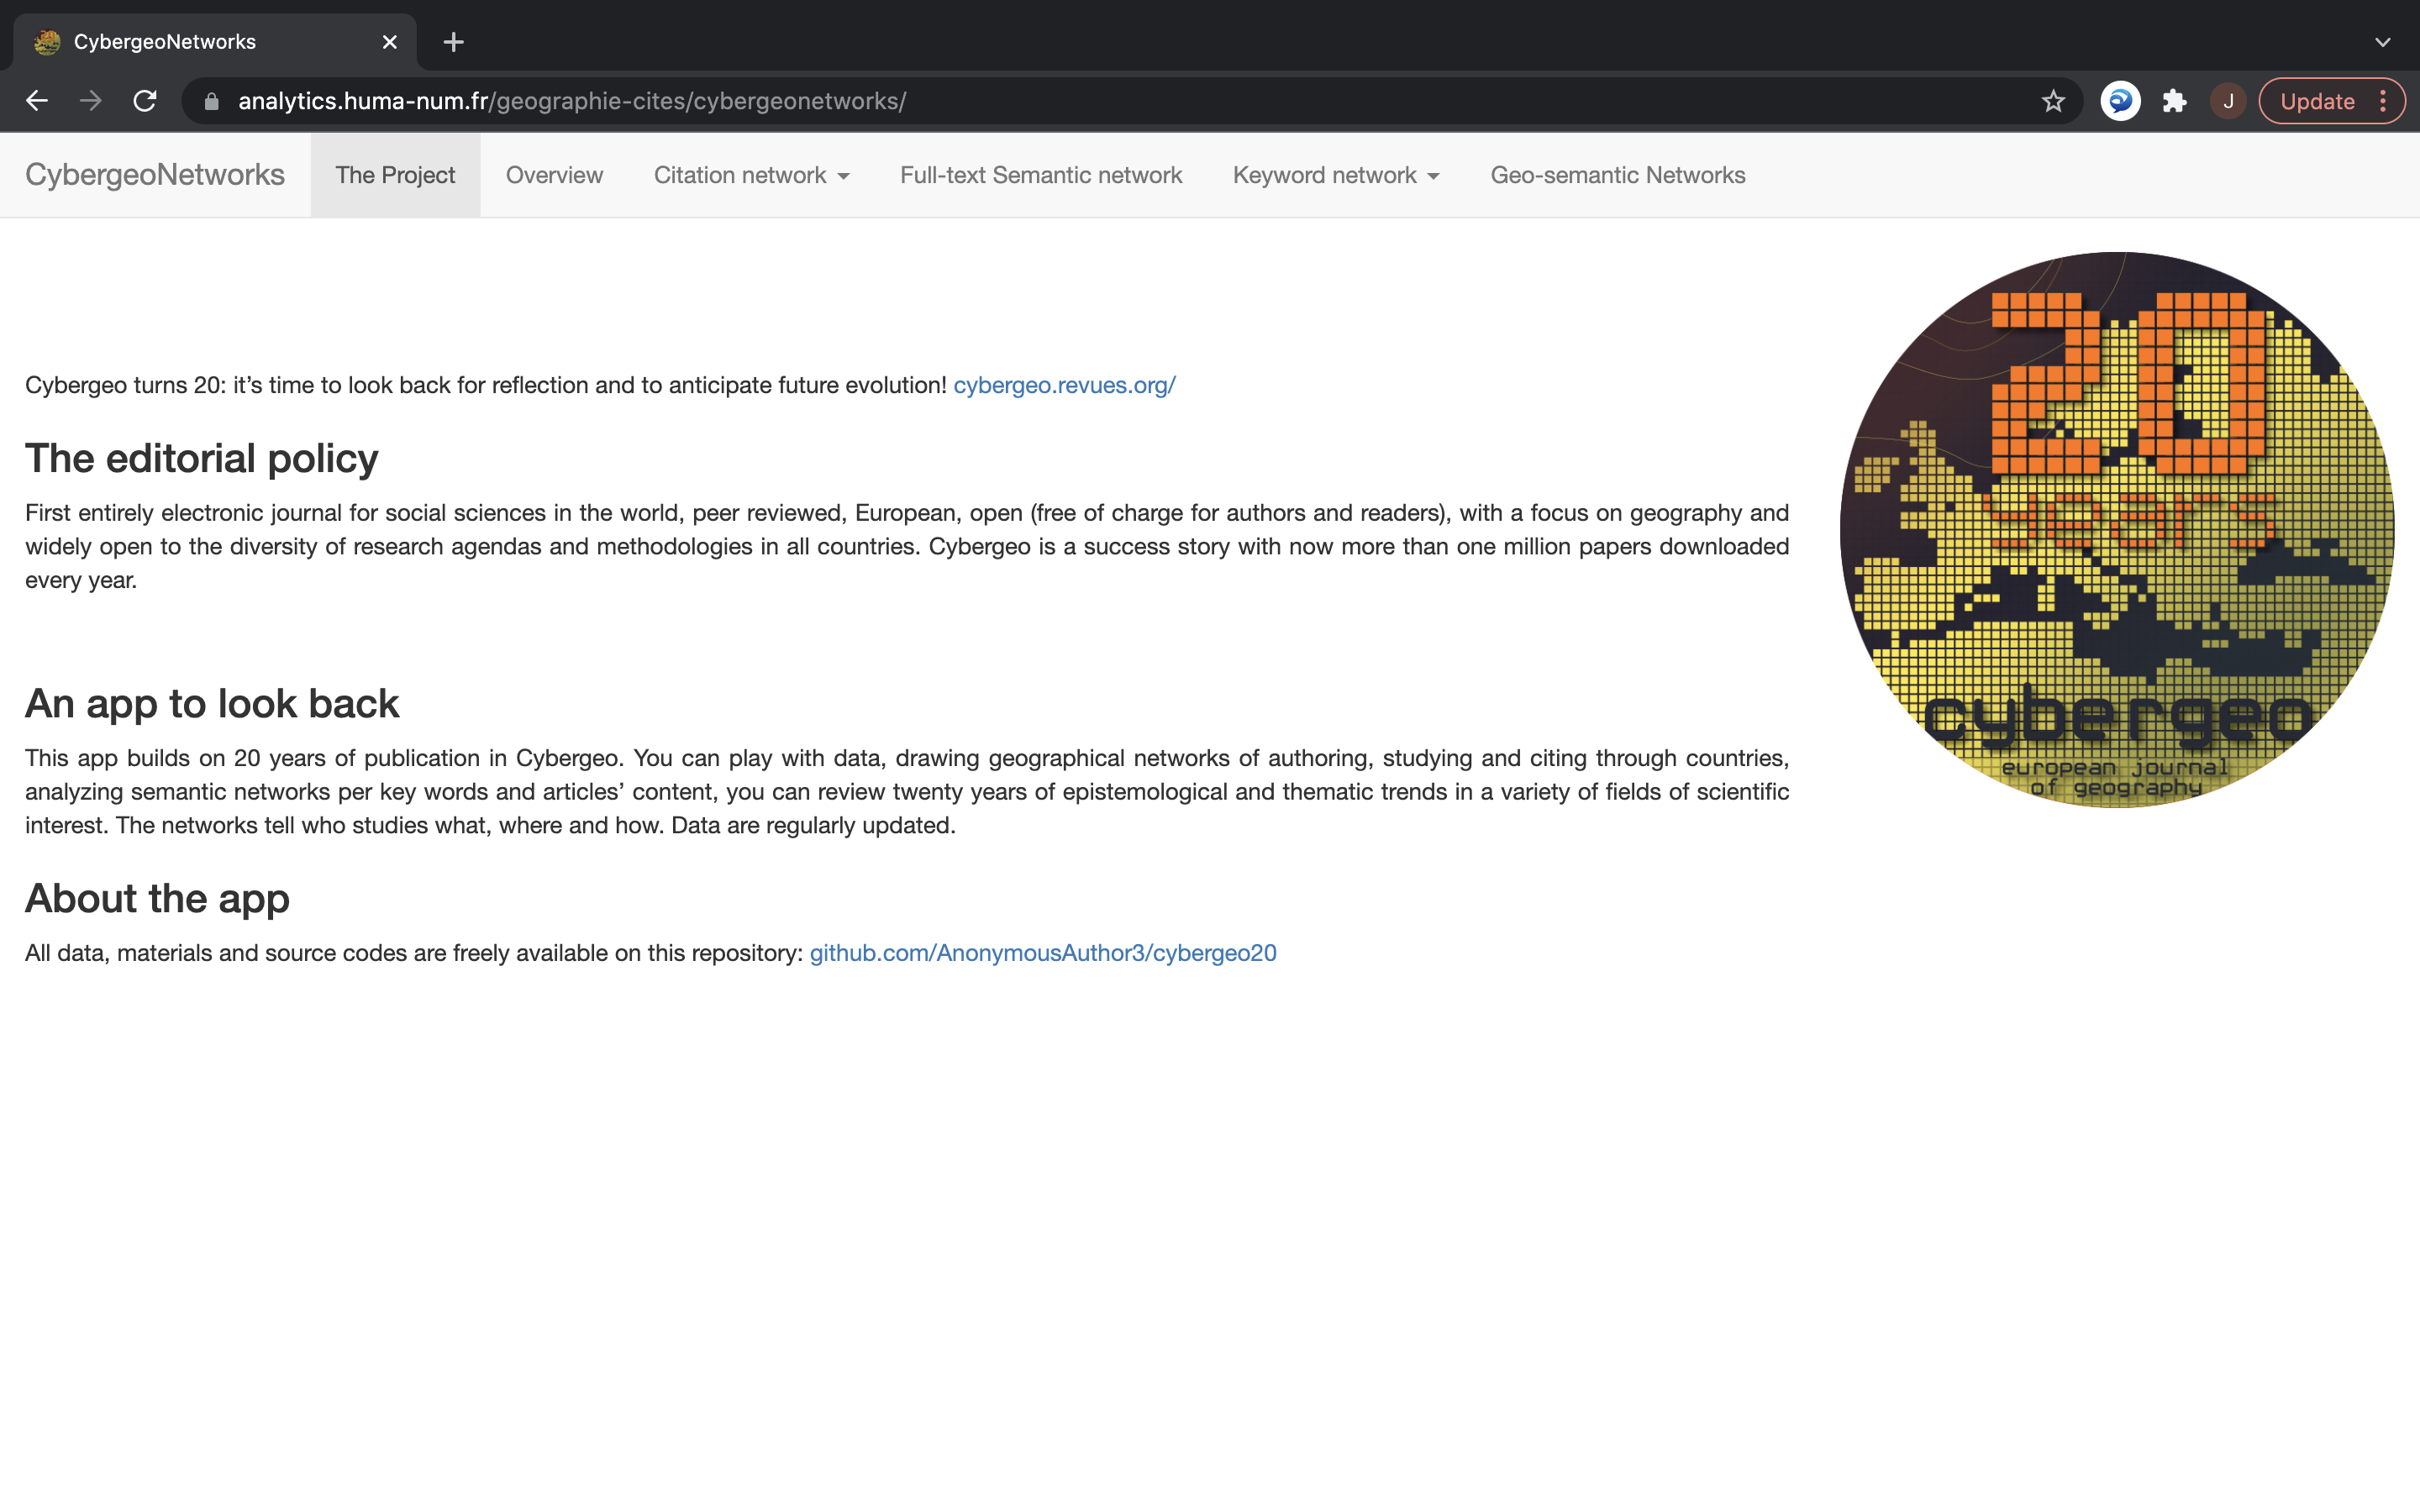
\includegraphics[width=0.7\linewidth]{figures/cyb_app.png}
\end{center}



\end{frame}



\begin{frame}
\frametitle{Favoriser la réflexivité}

% Reflexivite : publi EPB et scim

Analyses \textbf{multi-méthodes} de différents corpus : mots-clés, textes complets, voisinage de citations, contenu géographique \cite{raimbault2021empowering} \cite{raimbault2019exploration}

\medskip

$\rightarrow$ mise à disposition des lecteurs, auteurs et éditeurs d'outils pour se situer au sein des connaissances et ainsi aider à la réflexivité 

\begin{center}
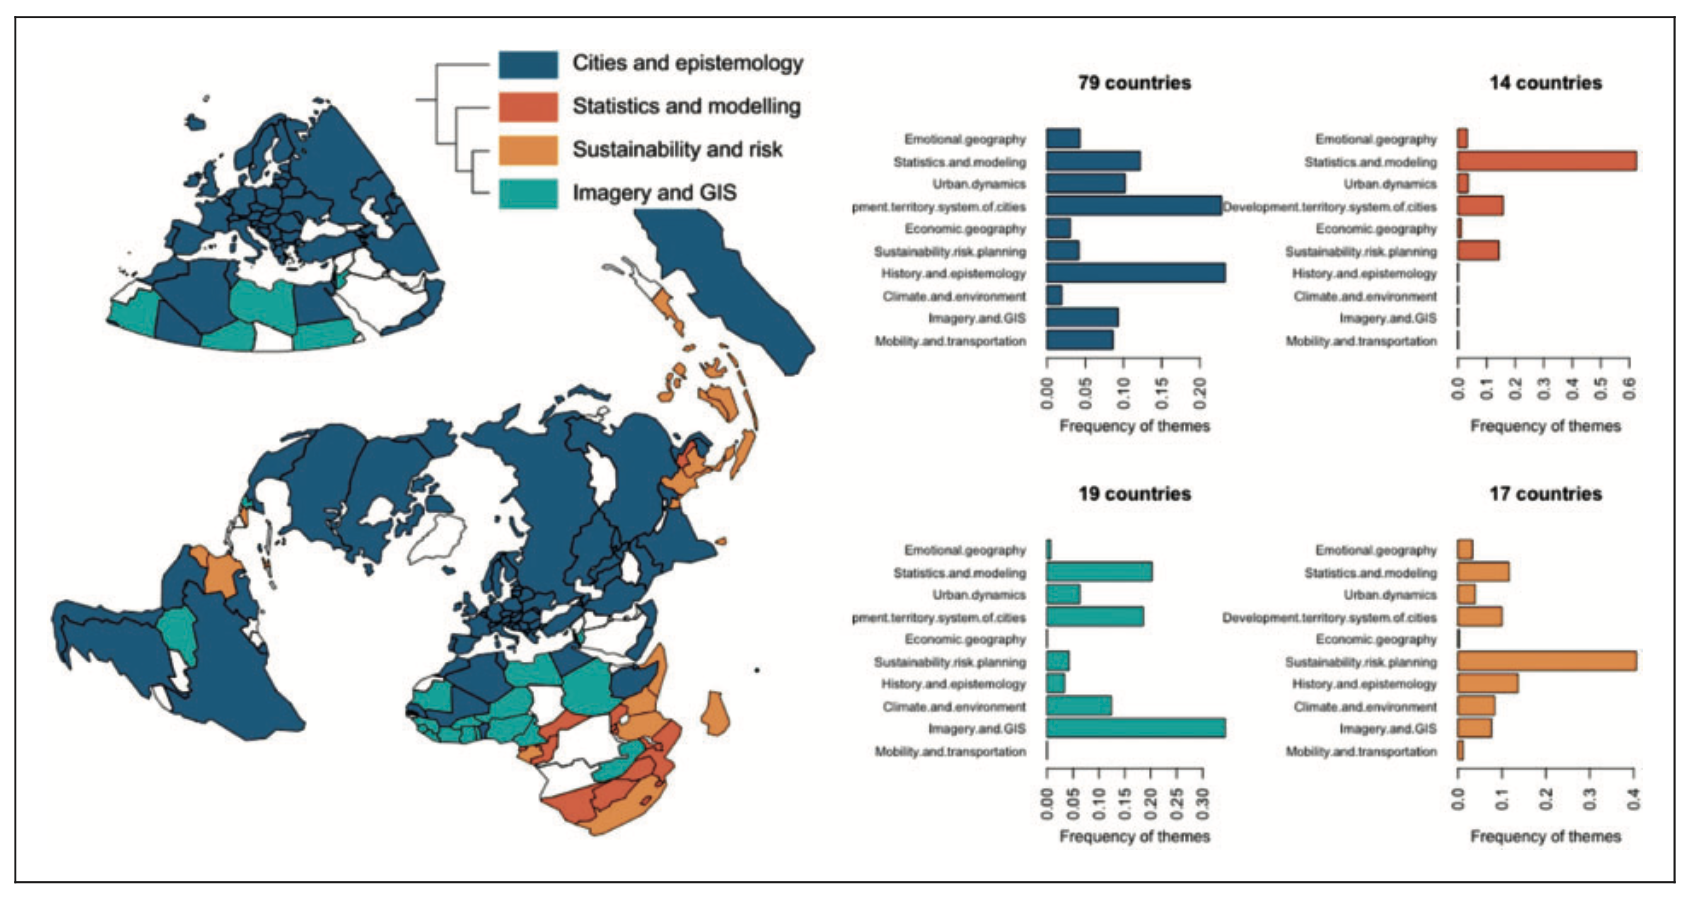
\includegraphics[width=0.55\linewidth]{figures/cyb_keywords.png}
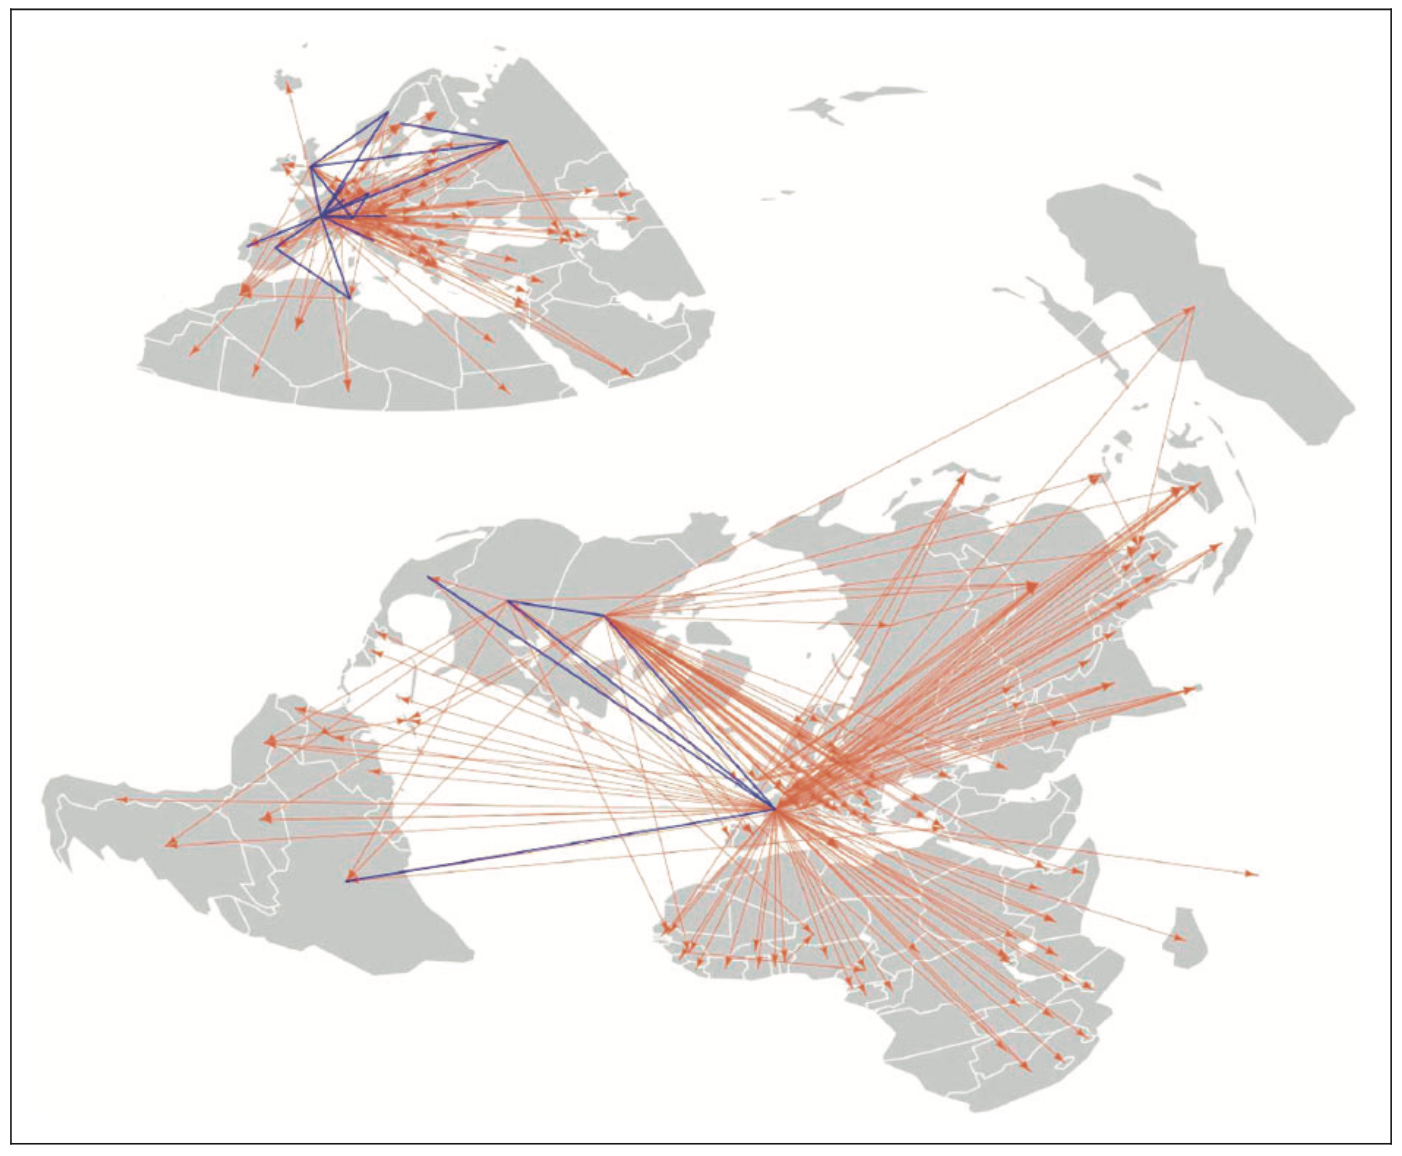
\includegraphics[width=0.35\linewidth]{figures/cyb_subject.png}
\end{center}

\end{frame}


\section{Vers une intégration des domaines de connaissance}


\begin{frame}
\frametitle{Vers une intégration des domaines de connaissance}

% slides Livet 2010 ; Raimbault 2017

La production de connaissances en \textbf{Géographie Théorique et Quantitative} implique une intégration forte entre \textbf{domaines de connaissance} \cite{livet2010ontology} \cite{raimbault2017applied}

\medskip

\begin{center}
	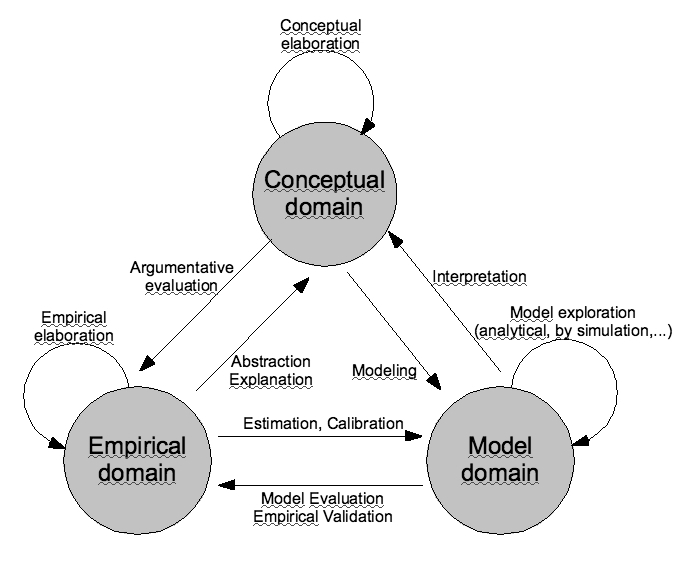
\includegraphics[height=0.42\textheight]{figures/Livet2010_Figure1.jpg}%\hspace{0.1cm}
	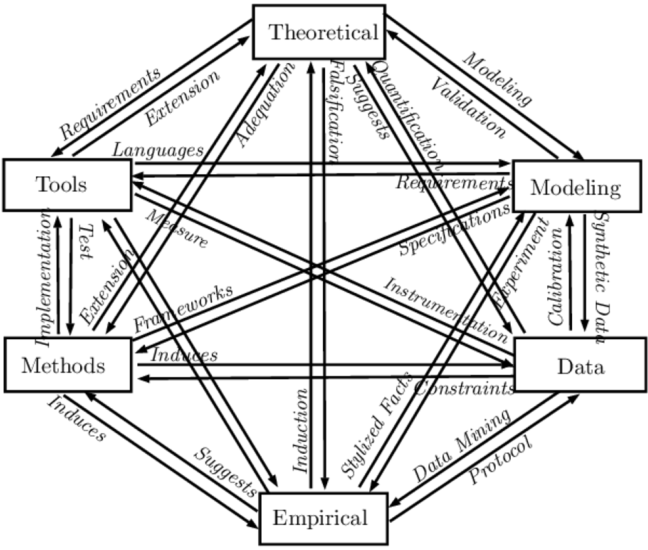
\includegraphics[height=0.42\textheight]{figures/framework.png}
\end{center}



\end{frame}


\begin{frame}
\frametitle{Quantification automatique des domaines de connaissance}

% tableau resultats TheoQuant

\begin{itemize}
	\item Cette intégration s'observe empiriquement sur des corpus de TQG (Loi de Zipf, Théorie évolutive des villes) \cite{raimbault2025mapping}
	\item Les nouvelles méthodes d'apprentissage profond augmentent la précision de classification jusqu'à 80\% \cite{raimbault2026classifying}
\end{itemize}

\medskip

\begin{center}

	
\begin{tabular}{l|ccc}
            \hline
            \textbf{Model} & \textbf{Accuracy} & \textbf{Macro F1} & \textbf{Weighted F1} \\
            \hline
            Zero-R (Baseline) & 0.393 ($\pm$0.03) & 0.141 ($\pm$0.01) & 0.223 ($\pm$0.03) \\ 
            TF-IDF + Logit    & 0.650 ($\pm$0.03) & 0.594 ($\pm$0.03) & 0.650 ($\pm$0.03) \\
            \textbf{SciBERT}  & \textbf{0.798 ($\pm$0.01)} & \textbf{0.743 ($\pm$0.03)} & \textbf{0.796 ($\pm$0.01)} \\
            \hline
        \end{tabular}

\end{center}


\end{frame}



\begin{frame}
\frametitle{Perspectives pour Cybergeo}

% slide speculatif avec propositions

% knowledge graph, web semantique

% instances OML - intégration auto?

%Expérimentations possibles 

Pistes d'expérimentations futures selon les besoins et opportunités :

\begin{itemize}
	\item Outil OpenJournalScope permettant une exploration des corpus spatialisés de revue, mis à jour en continu
	\item Méthodes IA pour une classification automatique des domaines de connaissance, et une explicitation de l'intégration des Model papers et Data papers au sein du corpus de la revue
	\item Interopérabilité, enrichissement automatique des métadonnées, construction de graphes de connaissance, peuplement d'ontologies pour le web sémantique
	\item Outils d'assistance à la modélisation : instances OpenMOLE liées aux articles GeOpenMod
\end{itemize}


\end{frame}


\section{Conclusion}


\begin{frame}
\frametitle{Une Science Ouverte appliquée aux mains des acteurs}

$\rightarrow$ Cybergeo a toujours été une revue pionnière pour la pratique de la Science Ouverte

\bigskip

$\rightarrow$ Mise en place de rubriques et développement d'outils permettant la reproductibilité et la réflexivité

\bigskip

$\rightarrow$ Une ambition renouvelée d'une \textbf{Science Ouverte Appliquée}, par et pour les acteurs de la science et en alternative aux éditeurs commerciaux


\end{frame}


%%%%%%%%%%%%%%%%%%%%%%%%%%%%%%%%
%\begin{frame}[allowframebreaks]
%\frametitle{References}
%\footnotesize
%\bibliographystyle{apalike}
%\bibliography{biblio}
%\end{frame}
%%%%%%%%%%%%%%%%%%%%%%%%%%%%%%%%

\begin{frame}{Bibliographie (1/3)}

\footnotesize

\begin{thebibliography}{}

\bibitem[Banos, 2014]{banos2014presentation}
Banos, A. (2014).
\newblock Présentation de geopenmod.
\newblock {\em Cybergeo: European Journal of Geography}.

\bibitem[Cybergeo, 2017]{cybergeo2017presentation}
Cybergeo (2017).
\newblock Présentation de la rubrique data papers.
\newblock {\em Cybergeo: European Journal of Geography}.

\bibitem[Livet et~al., 2010]{livet2010ontology}
Livet, P., Muller, J.-P., Phan, D., and Sanders, L. (2010).
\newblock Ontology, a mediator for agent-based modeling in social science.
\newblock {\em Journal of Artificial Societies and Social Simulation}, 13(1):3.


\end{thebibliography}

\end{frame}

\begin{frame}{Bibliographie (2/3)}

\footnotesize

\begin{thebibliography}{}
    \bibitem[Raimbault, 2017]{raimbault2017applied}
Raimbault, J. (2017).
\newblock An applied knowledge framework to study complex systems.
\newblock In {\em Complex Systems Design \& Management}, pages 31--45.

\bibitem[Raimbault, 2019]{raimbault2019exploration}
Raimbault, J. (2019).
\newblock Exploration of an interdisciplinary scientific landscape.
\newblock {\em Scientometrics}, 119(2):617--641.

\bibitem[Raimbault, 2025]{raimbault2025mapping}
Raimbault, J. (2025).
\newblock Mapping the integration between knowledge domains in theoretical and
  quantitative geography.
\newblock In {\em ECTQG 2025}.


\end{thebibliography}

\end{frame}


\begin{frame}{Bibliographie (3/3)}

\footnotesize

\begin{thebibliography}{}

\bibitem[Raimbault, 2026]{raimbault2026classifying}
Raimbault, J. (2026).
\newblock Classifying knowledge domains of theoretical and quantitative
  geography publications.
\newblock In {\em TheoQuant 2026}.

\bibitem[Raimbault et~al., 2021]{raimbault2021empowering}
Raimbault, J., Chasset, P.-O., Cottineau, C., Commenges, H., Pumain, D.,
  Kosmopoulos, C., and Banos, A. (2021).
\newblock Empowering open science with reflexive and spatialised indicators.
\newblock {\em Environment and Planning B: Urban Analytics and City Science},
  48(2):298--313.

\bibitem[Reuillon et~al., 2013]{reuillon2013openmole}
Reuillon, R., Leclaire, M., and Rey-Coyrehourcq, S. (2013).
\newblock Openmole, a workflow engine specifically tailored for the distributed
  exploration of simulation models.
\newblock {\em Future Generation Computer Systems}, 29(8):1981--1990.




\end{thebibliography}

\end{frame}













\end{document}

